\documentclass{standalone}

\usepackage{graphicx}

\usepackage{tikz}

\usetikzlibrary{positioning}
\usetikzlibrary{arrows.meta}
\usetikzlibrary{calc}

\begin{document}

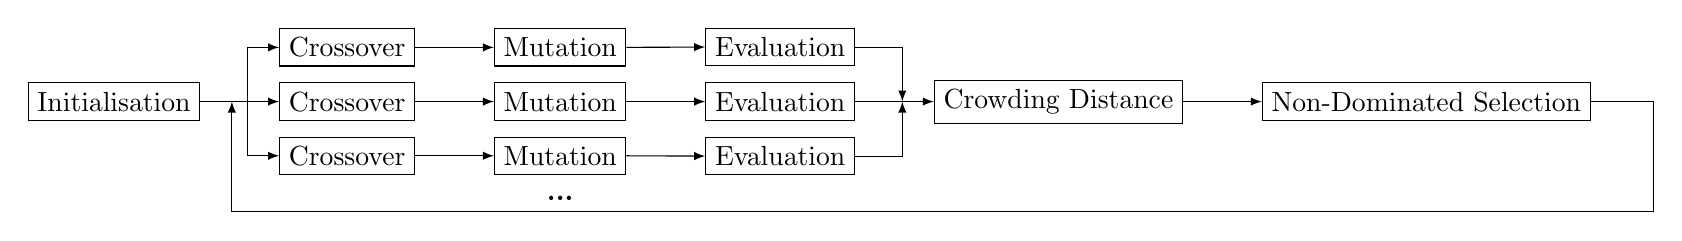
\begin{tikzpicture}[
    block/.style={rectangle, draw=black, fill=white},
]
    \node[block] (B1) [] {Initialisation};

    \node[block] (BA2) [right=of B1] {Crossover};
    \node[block] (BA3) [right=of BA2] {Mutation};
    \node[block] (BA4) [right=of BA3] {Evaluation};

    \node[block] (BB2) [above=0.2cm of BA2] {Crossover};
    \node[block] (BB3) [above=0.2cm of BA3] {Mutation};
    \node[block] (BB4) [above=0.2cm of BA4] {Evaluation};

    \node[block] (BC2) [below=0.2cm of BA2] {Crossover};
    \node[block] (BC3) [below=0.2cm of BA3] {Mutation};
    \node[block] (BC4) [below=0.2cm of BA4] {Evaluation};

    \node[] () [below=0.15cm of BC3] {\textbf{...}};

    \node[block] (B5) [right=of BA4] {Crowding Distance};
    \node[block] (B6) [right=of B5] {Non-Dominated Selection};

    \draw[] (B1.east) -- ($(B1.east)+(0.6,0)$);
    \draw[-latex] ($(B1.east)+(0.6,0)$) -| ($(BA2.west)+(-0.4,0)$) -- (BA2.west);
    \draw[-latex] ($(B1.east)+(0.6,0)$) -| ($(BB2.west)+(-0.4,0)$) -- (BB2.west);
    \draw[-latex] ($(B1.east)+(0.6,0)$) -| ($(BC2.west)+(-0.4,0)$) -- (BC2.west);

    \draw[-latex] (BA2.east) -- (BA3.west);
    \draw[-latex] (BA3.east) -- (BA4.west);

    \draw[-latex] (BB2.east) -- (BB3.west);
    \draw[-latex] (BB3.east) -- (BB4.west);

    \draw[-latex] (BC2.east) -- (BC3.west);
    \draw[-latex] (BC3.east) -- (BC4.west);
    
    \draw[-latex] (B5.east) -- (B6.west);

    \draw[] (BA4.east) -| ($(B5.west)+(-0.4,0)$);
    \draw[-latex] (BB4.east) -| ($(B5.west)+(-0.4,0)$);
    \draw[-latex] (BC4.east) -| ($(B5.west)+(-0.4,0)$);

    \draw[-latex] ($(B5.west)+(-0.4,0)$) -- (B5.west);

    \draw[-latex] (B6.east) -| ($(B6.east)+(0.8,-1.4)$) -| ($(B1.east)+(0.4,-1.4)$) -- ($(B1.east)+(0.4,0)$);
\end{tikzpicture}

\end{document}